\documentclass[final,hyperref={pdfpagelabels=false},notitlepage=true]{beamer} 
\usepackage{times}
\usepackage{listings}
\usepackage{amsmath,amssymb}
\usepackage[english]{babel}
\usepackage[latin1]{inputenc}
\usepackage[orientation=portrait,size=a0,scale=1.4,debug]{beamerposterbuiltin}   % e.g. for DIN-A0 poster
%\usepackage[size=custom,width=200,height=120,scale=2,debug]{beamerposter}  % e.g. custom size poster
% ...
\usepackage{xspace}
\usepackage{fp}
\usepackage{ifthen}

\useoutertheme{default}
\useoutertheme{hipinfolines}
\useinnertheme{rounded}

\title[]{\Huge Using Git Distributed Version Control Tool to Manage a HEP Data Analysis Project}

\author{A. Heikkinen\inst{1}, \underline{P. Kaitaniemi\inst{1,2}}}

\institute[] % (optional, but mostly needed)
{
  \inst{1}%
  Helsinki Institute of Physics P.O.Box 64 (Gustaf H\"allstr\"omin katu 2), FIN-00014 University of Helsinki, Finland
  \\
  \inst{2}%
  CEN-Saclay, CEA-IRFU/SPhN, 91 191 Gif sur Yvette, France
}

\date[March 12th, 2009]{March 12th, 2009}

\begin{document}
  \begin{frame}{} 
    \begin{center}
    \maketitle
    \end{center}
    \vfill
    \begin{abstract}
Version control allows software developers to keep track of project history in
a systematic and detailed manner. 
%The project can be a data analysis or simulation program source code, 
%or even LaTeX code of a paper or thesis. 
In addition to tracking history, version control tools allow
one to merge contributions between several authors.
% background
Recently CERN has chosen to upgrade centralised CVS version control
system \cite{cernsvn} to another modernised centralised system called Subversion (SVN) \cite{svnsite}.
Unfortunately it does not offer the flexibility of the
distributed systems we are interested in. 

Git, a distributed version control tool \cite{torvalds}, however, 
provides this flexibility, 
and can be used as a ``super client'' with the CERN SVN service.
We discuss advantages of distributed version control tools,
such as Git, over traditional centralised ones. 
Most significant advantage is that the distributed
tools don't need a central server, and users can utilise
version control locally on their own computers without
heavy support infrastructure.
% our case and example image
We present an example use case for Git in a HEP data analysis and publication writing project (Fig.~1)~\cite{pk09aProceedings}.
We also demonstrate how to use Git
together with CERN central SVN version control for high energy physics data
analysis software maintenance.

    \end{abstract}
    \begin{columns}[t]
      \begin{column}{0.45\linewidth}

    \begin{block}{\large Abstract}
      Distributed version control.
    \end{block}

    \begin{block}{\large Version history}
      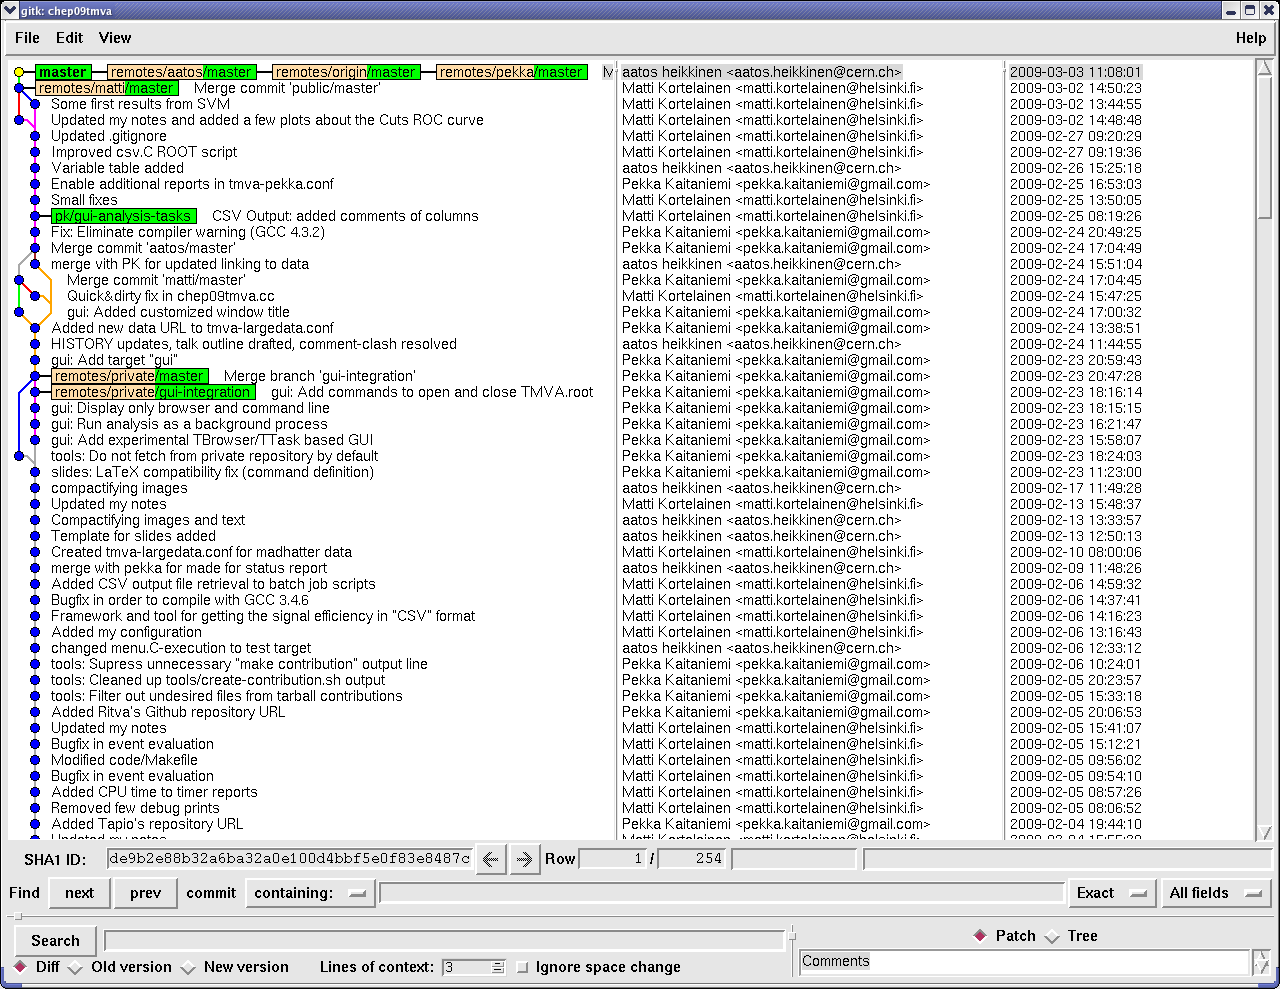
\includegraphics[scale=1.0]{images/gitk-history.png}
    \end{block}

    \begin{block}{\large Git GUI, graphical commit tool}
      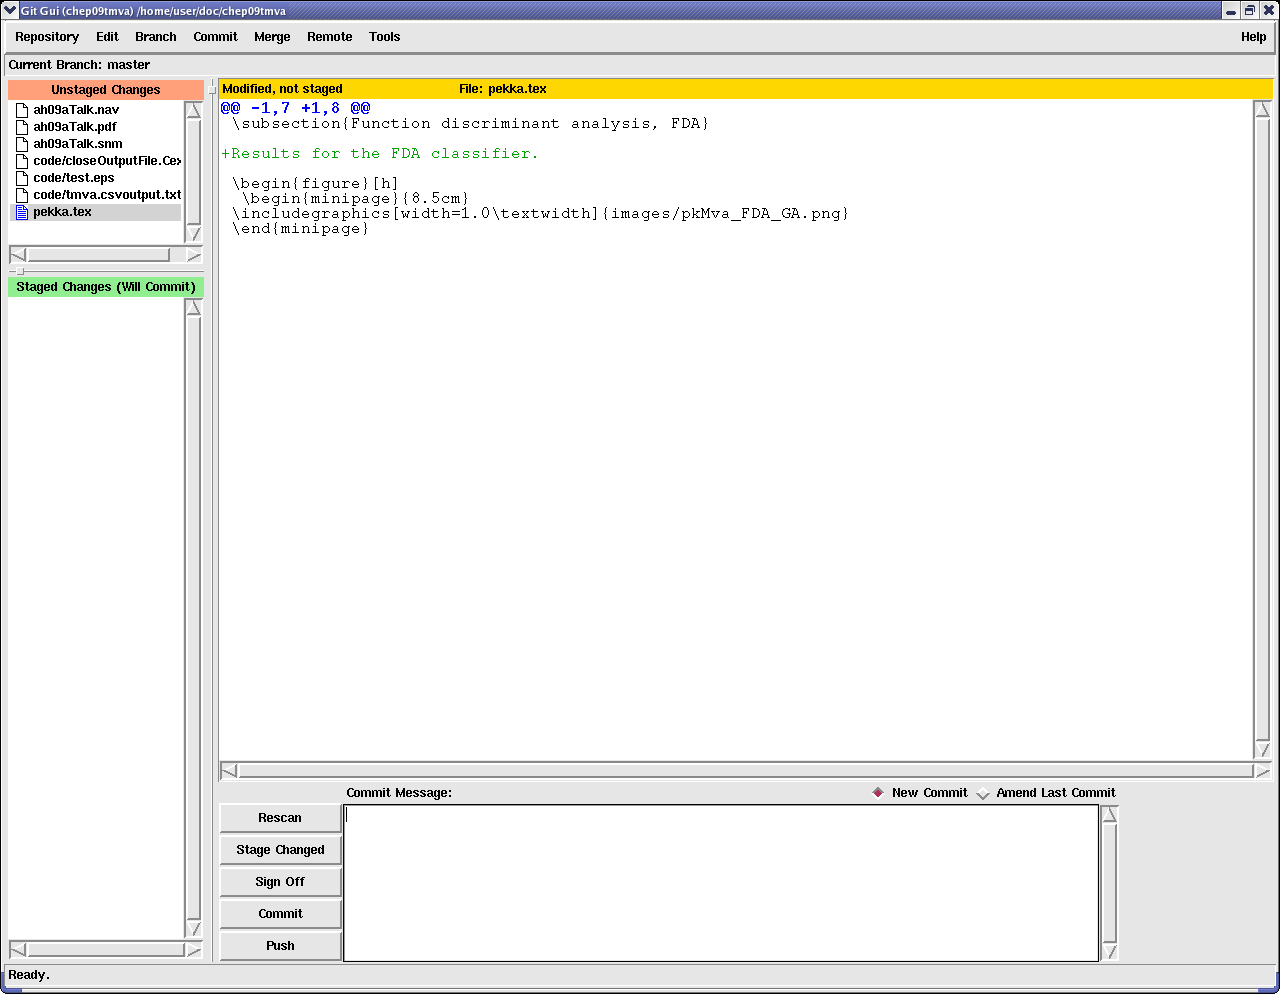
\includegraphics[scale=1.0]{images/gui-screenshot.png}
    \end{block}

    \begin{block}{\large Git GUI Blame}
      Find out who is responsible for each line of code/text. Unique
      feature of Git blame is that it can heuristically find similar
      content in other files that are part of the project thus
      allowing us to track content history beyond file boundaries.
      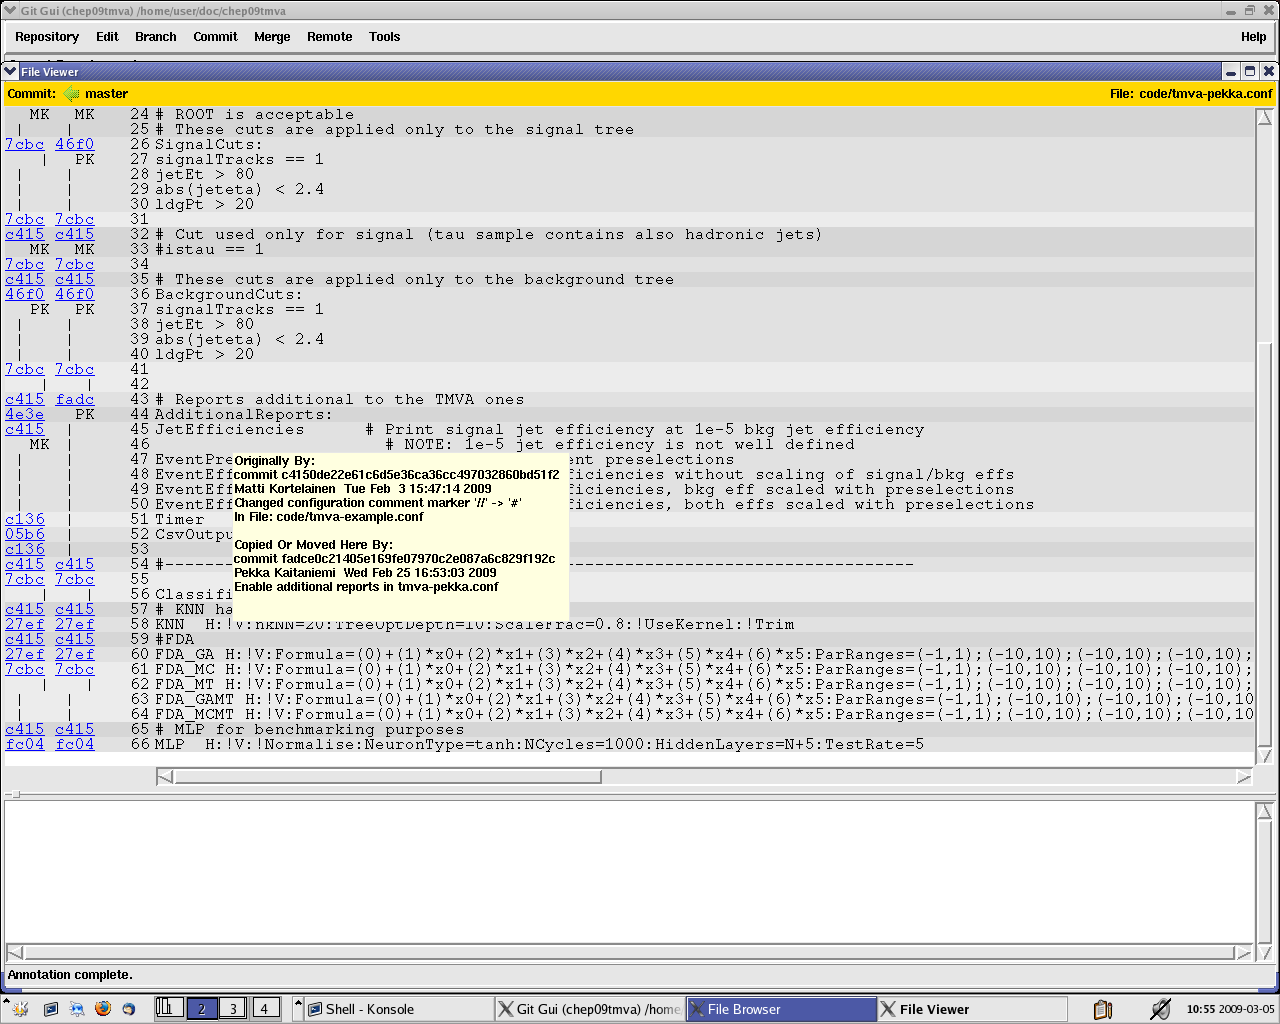
\includegraphics[scale=1.0]{images/git-gui-blame-content-copy-detection.png}
    \end{block}

    \begin{block}{\large Subversion}

    \end{block}

    \end{column}
      \begin{column}{0.45\linewidth}
    \begin{block}{\large Fontsizes}
      \centering
      {\tiny tiny}\par
      {\scriptsize scriptsize}\par
      {\footnotesize footnotesize}\par
      {\normalsize normalsize}\par
      {\large large}\par
      {\Large Large}\par
      {\LARGE LARGE}\par
      {\veryHuge veryHuge}\par
      {\VeryHuge VeryHuge}\par
      {\VERYHuge VERYHuge}\par
    \end{block}

\begin{block}{\large Bibliography}
%%%
%%% The bibliography: the references are listed here.
%%%
\begin{thebibliography}{9}
\bibitem{cernsvn}
\href{http://cern.ch/svn}{CERN central SVN service (http://cern.ch/svn)}

\bibitem{svnsite}
\href{http://subversion.tigris.org}{Subversion website (http://subversion.tigris.org)}

\bibitem{torvalds}
L.Torvalds with the Linux kernel team,
Git Version Control System website,
\href{http://git-scm.com/}{http://git-scm.com/}

%\bibitem{gitsite} % same as \bibitemtorvalds
%\href{http://git.or.cz}{Git website (http://git.or.cz)}%

\bibitem{pk09aProceedings}
P.~Kaitaniemiemi and A.~Heikkinen et al.,
Ideal $\tau$-tagging with TMVA multivariate data-analysis toolkit,
Proceedings of International Conference on 
Computing in High Energy and Nuclear Physics, CHEP'09
(To be published)

\end{thebibliography}
\end{block}
    \vfill
    \end{column}
    \end{columns}
  \end{frame}
\end{document}
%%%%%%%%%%%%%%%%%%%%
%%% Local Variables: 
%%% mode: latex
%%% TeX-PDF-mode: t
%%% End: 
